%  !TeX spellcheck = en_GB
%  WangSheying于2015/11/2整理,TJU北洋园校区
%  TeXLive2015+TeXstudio个人推荐,可在线升级usepackage,比较方便
%*****************************************************************************************
%  从这里开始到\begin{document}是导言区,称之为preamble
\documentclass[UTF8]{beamer}
\usepackage[fontset=mac]{ctex}
%\usepackage[UTF8]{ctex}                 %使用中文要添加,可解决中文文档输入
\usepackage{newtxtext,newtxmath}  %字重齐全的高质量数学字体
\usepackage{mathrsfs}             %大写ABC的花体使用命令是\mathscr{}
\usepackage{caption}
\usepackage{subcaption}
\usepackage{graphicx}             %添加图片
\usepackage{bm}                   %专门处理数学粗体的bm宏包,使用命令是\bm{}
\usepackage{extarrows}            %延长符号,可在=,->等符号加多个字母
%\usepackage{amstext}              %它定义命令 \text,可用于在数学公式中插入少量文本,并可调整上下标中文本字体的尺寸。
\usepackage{amsthm}               %它定义了一个 proof 环境,用来排版定理和证明,能自动在最后添加证毕符号。它还提供一个命令:\newtheorem{定理环境名}{标题}[计数器名],可自定义定理类 环境
\usefonttheme{professionalfonts}  %这个更好看些,数学字体
\usepackage{indentfirst}          %首行缩进
\usepackage{verbatim}
\usepackage{amsmath}
\usepackage{amsfonts}
\usepackage{amssymb}
\usepackage{xcolor}
%\usepackage{subfigure}
\usepackage[english]{babel}
\usepackage{algorithm}
\usepackage{algorithmic}
\usepackage{tikz}
\setlength{\parindent}{2em}      %首行缩进2字符
\setbeamertemplate{theorems}[numbered]
\setbeamertemplate{caption}[numbered]
%******************************************************************************************
%            以上是各种宏包
%******************************************************************************************
%下面是定理,定义,引言的声明,可自行添加

\newtheorem{thm}{Theorem}
\newtheorem{lem}[thm]{Lemma}
\newtheorem{cor}[thm]{Corollary}
\newtheorem{prop}[thm]{Proposition}
\newtheorem{defi}[thm]{Definition}
\newtheorem{remark}[thm]{Remark}
\newtheorem{claim}[thm]{Claim}

\newenvironment{proofnoqed}{\begin{proof}<span style="background-color: rgb(255, 0, 0);">\renewcommand{\qedsymbol}{}  }{\end{proof} }
%有的证明比较长,前面的应该没有证毕符号,只在最后一个用proof,其他应该用自定义的新环境proofnoqed



%  三种颜色   red  purple   magenta





%上面是定理,定义,引言的声明,可自行添加
%******************************************************************************************
%下面是beamer的主题设置,目录框架结构,其实就是标题,目录等在上下左右哪一个位置放置,以及目录怎么显示
\usetheme{Singapore}            % 幻灯片模板选择singapore
\usecolortheme{sidebartab}      % 幻灯片模板的色彩sidebartab

\AtBeginSection[]{              % 幻灯片框架% 在每个Section前都会加入的Frame,
	\begin{frame}[plain]
		\frametitle{Outline}
		\tableofcontents[sectionstyle=show/shaded,subsectionstyle=show/show/shaded]
	\end{frame} 
}
%  \tableofcontents[comma-separated option list]具体讲解见《The beamer class User Guide》,
%  http://texdoc.net/texmf-dist/doc/latex/beamer/doc/beameruserguide.pdf     See in section 10.5 Adding a table of contents.
%  section和subsection相互独立,显示效果互不相关,Allowed ⟨styles⟩ are show, shaded, and hide
%  sectionstyle=⟨style for current section⟩/⟨style for other sections⟩
%  subsectionstyle=⟨style for current subsection⟩/⟨style for other subsections in current section⟩/⟨style for subsections in other sections⟩
%
% 上面是beamer的主题设置,目录框架结构,其实就是标题,目录等在上下左右哪一个位置放置,以及目录怎么显示
%*******************************************************************************************
%       下面标题页的内容设置,根据实际情况修改即可
\title{The Design and Implementation of Kafka}  % 幻灯片封面
\author{Wang Sheying}
\institute{HuiLongGuan of Beijing}
\date{\today}  

%\date{9月 23, 2019}%一般是\today
%      上面标题页的内容设置根据实际情况修改即可
%*******************************************************************************************
%  \begin{document}以上是导言区,称之为preamble
%*******************************************************************************************
\begin{document}
	\begin{frame}[plain]
		%plain格式使得一帧的最上面是白色的,没有plain,会有色彩
		\titlepage
	\end{frame}
	\begin{frame}[plain]               % 幻灯片目录
		\frametitle{Outline}
		\tableofcontents[sectionstyle=show/show,subsectionstyle=show/show/hide]
	\end{frame}
	%The beamer class这本小册子有目录格式的讲解,sectionstyle,subsectionstyle都有,P100页
	%User Guide for version 3.36. 文档可在google搜索The beamer class,即可得到
%  以上是标准的配置,还有最下面的一部分标准配置
%********************************************************************************************
%    一帧的具体格式样例参考
%\section{节的名字}
%\subsection{小节的名字}
%\begin{frame}[plain,t]{节的名字} %也可以使用\frametitle{节的名字}效果一样
%	\structure{小节的名字} \\  \vspace{2ex}
%	节的名字正上方居中,小节的名字紧下方居左。
%\end{frame}
%*********************************************************************************************
%                  下面就是正文,自己的内容
%*********************************************************************************************

\section{Introduction}
\begin{frame}[plain,t]{Introduction} %也可以使用\frametitle{节的名字}效果一样
	%\structure{} \\
	  \vspace{2ex}

   Apache Kafka is used for building real-time data pipelines and streaming apps. 
    
 \vspace{-2ex}
\begin{figure}
    \centering
    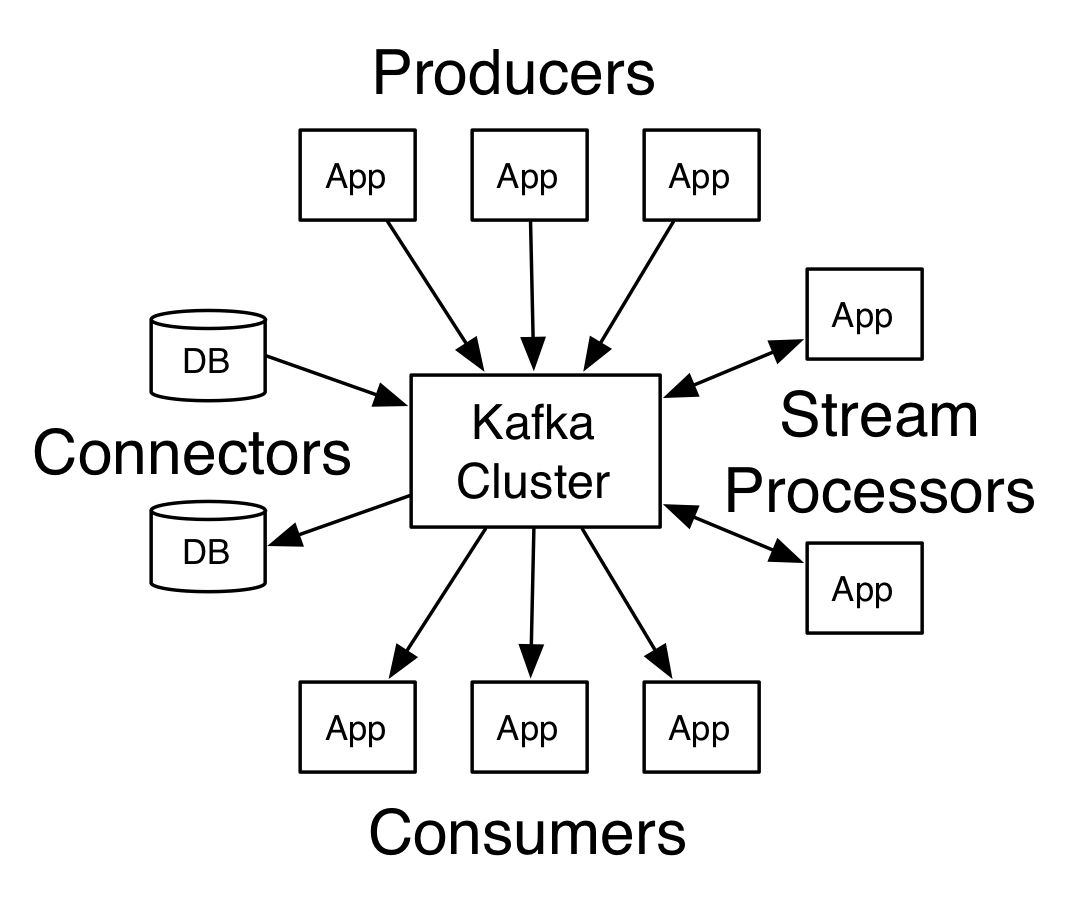
\includegraphics[width=0.7\linewidth]{image/0101}
    %\caption{}
    \label{fig:0101}
\end{figure}
\end{frame}



\begin{frame}[plain,t]{Introduction} %也可以使用\frametitle{节的名字}效果一样
    %\structure{} \\
    \vspace{2ex}
    
    The Features of the Kafka
     \vspace{2ex}
    \begin{itemize}
        \item high throughput
        \item low latency
        \item high reliability
        \item high concurrency
        \item scalable horizontally
    \end{itemize}


    
\end{frame}
\begin{frame}[plain,t]{Introduction} %也可以使用\frametitle{节的名字}效果一样
    %\structure{} \\
    \vspace{2ex}
The popular use cases for Apache Kafka
 \vspace{2ex}
     \begin{itemize}
        \item messaging
        \item log aggregation
        \item stream processing
        \item website activity tracking
        \item metrics
    \end{itemize}
    
    
    
\end{frame}


\section{Producer}


\begin{frame}[plain,t]{Producer} %也可以使用\frametitle{节的名字}效果一样
    \structure{Architecture} \\
    \vspace{2ex}
    \begin{figure}
        \centering
        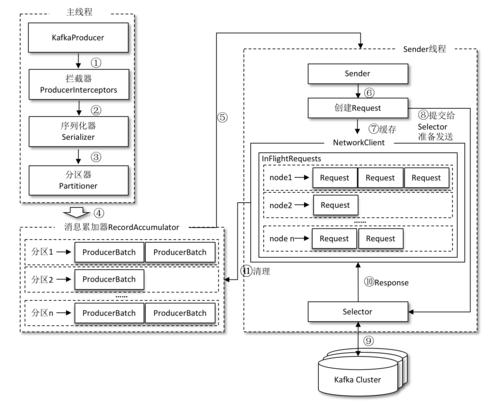
\includegraphics[width=0.8\linewidth]{image/0203}
        %\caption{}
        \label{fig:0203}
    \end{figure}
    

\end{frame}
\begin{frame}[plain,t]{Producer} %也可以使用\frametitle{节的名字}效果一样
    \structure{Encapsulation} \\
    \vspace{2ex}
    \begin{center}
        ProducerRecord(Main Thread) \\
        $\Downarrow$ \\
        ProducerBatch (Sender Thread) \\
        $\Downarrow$ \\
        <Partition, Deque<ProducerBatch>{}>(Sender Thread) \\
        $\Downarrow$ \\
        <Node, List<ProducerBatch>{}>(Sender Thread) \\
        $\Downarrow$ \\
        <Node, Request>(Sender Thread) \\
        {\color{red}$\Downarrow$} \\
        Broker(page cache) \\
        $\Downarrow$ \\
        Broker(log segment)
    \end{center}
    
\end{frame}
\begin{frame}[plain,t]{Producer} %也可以使用\frametitle{节的名字}效果一样
    \structure{Asynchronous Send} \\
    \vspace{2ex}
    The send() method is asynchronous.
    \begin{figure}
        \centering
        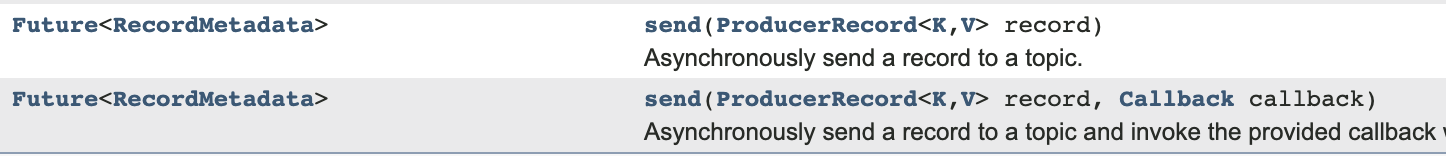
\includegraphics[width=0.8\linewidth]{image/0204}
        %\caption{}
        \label{fig:0204}
    \end{figure}

The acks config controls the criteria under which requests are considered complete.

\vspace{2ex}
 From Kafka 0.11, the KafkaProducer supports two additional modes: 
\begin{itemize}
    \item  the idempotent producer
    \item the transactional producer
\end{itemize}
\end{frame}
\begin{frame}[plain,t]{Producer} %也可以使用\frametitle{节的名字}效果一样
    \structure{Asynchronous Send} \\
    \vspace{2ex}
   

    \begin{figure}
        \centering
        \subcaptionbox{ordering of messages}[0.9\linewidth]{
            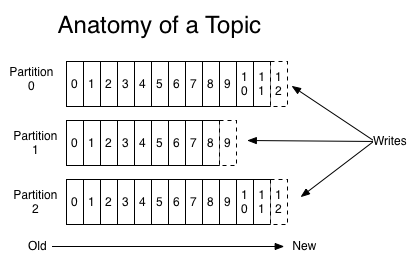
\includegraphics[width=0.48\linewidth]{image/0102}\quad
            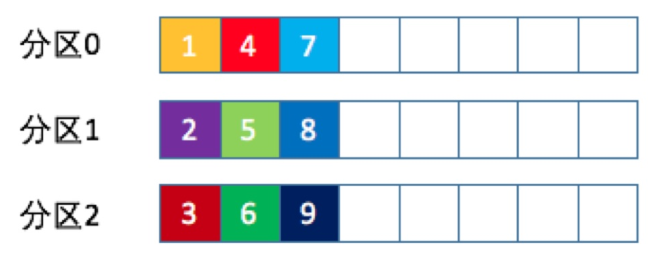
\includegraphics[width=0.48\linewidth]{image/0105}
        }

        %\caption{}
        \label{fig:0102}
    \end{figure}
\end{frame}

\begin{frame}[plain,t]{Producer} %也可以使用\frametitle{节的名字}效果一样
    \structure{Message Format} \\
    \vspace{2ex}
The following is the on-disk format of a RecordBatch.
\vspace{-1ex}
\begin{figure}
    \centering
    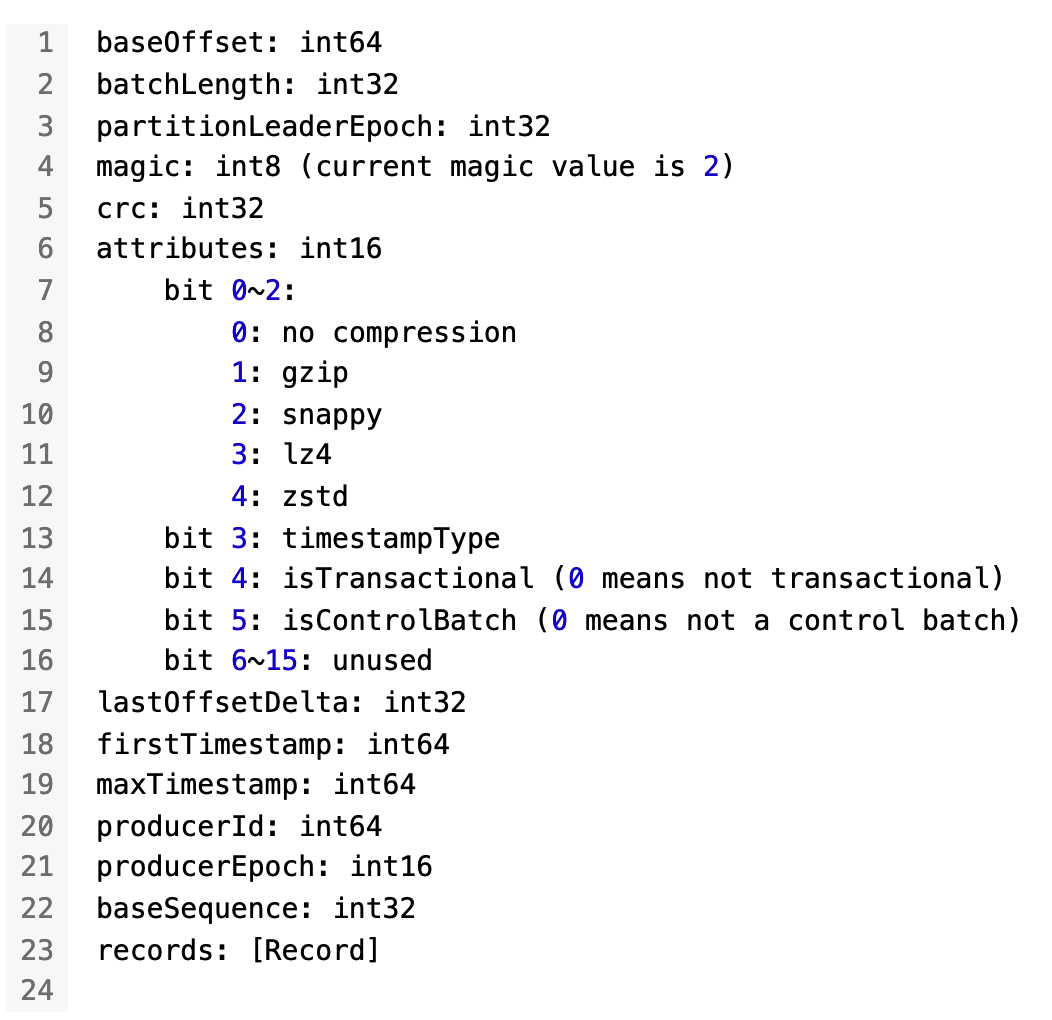
\includegraphics[width=0.65\linewidth]{image/0302}
    %\caption{}
    \label{fig:0302}
\end{figure}
\end{frame}
\begin{frame}[plain,t]{Producer} %也可以使用\frametitle{节的名字}效果一样
    \structure{Message Format} \\
    \vspace{2ex}
    The on-disk format of a record with Headers is delineated below.
    \begin{figure}[htbp]
        \centering
        \begin{minipage}[t]{0.48\textwidth}
            \centering
            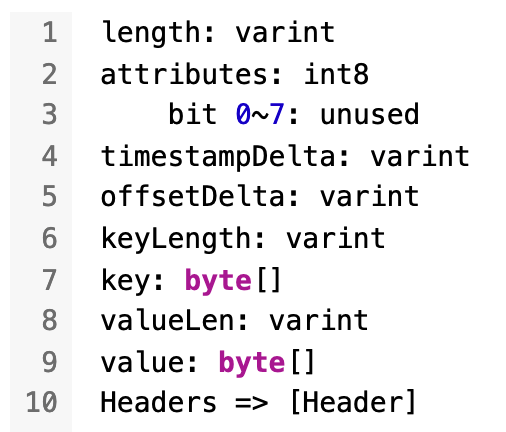
\includegraphics[width=0.8\linewidth]{image/0303}
            %\includegraphics[width=6cm]{test1.jpg}
            %\caption{World Map}
        \end{minipage}
        \begin{minipage}[t]{0.48\textwidth}
            \centering
            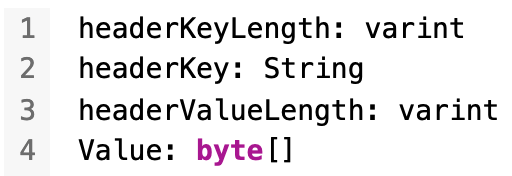
\includegraphics[width=0.8\linewidth]{image/0304}
            %\includegraphics[width=6cm]{test2.jpg}
            %\caption{Concrete and Constructions}
        \end{minipage}
    \end{figure}
\end{frame}


\section{Broker}
\begin{frame}[plain,t]{Broker} %也可以使用\frametitle{节的名字}效果一样
    \structure{Architecture} \\
    \vspace{2ex}
 The threading model is a single acceptor thread and N processor threads which handle a fixed number of connections each. 

 \vspace{2ex}
\begin{figure}
    \centering
    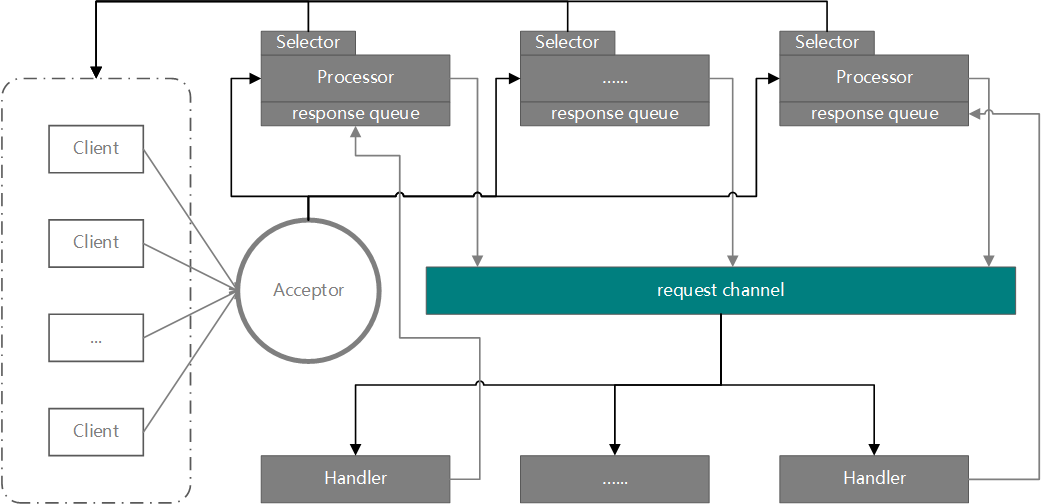
\includegraphics[width=0.9\linewidth]{image/0301}
    %\caption{}
    \label{fig:0301}
\end{figure}
    
\end{frame}
\begin{frame}[plain,t]{Broker} %也可以使用\frametitle{节的名字}效果一样
    \structure{Log} \\
    \vspace{2ex}
 Each log file is named with the offset of the first message it contains.
\begin{figure}
    \centering
    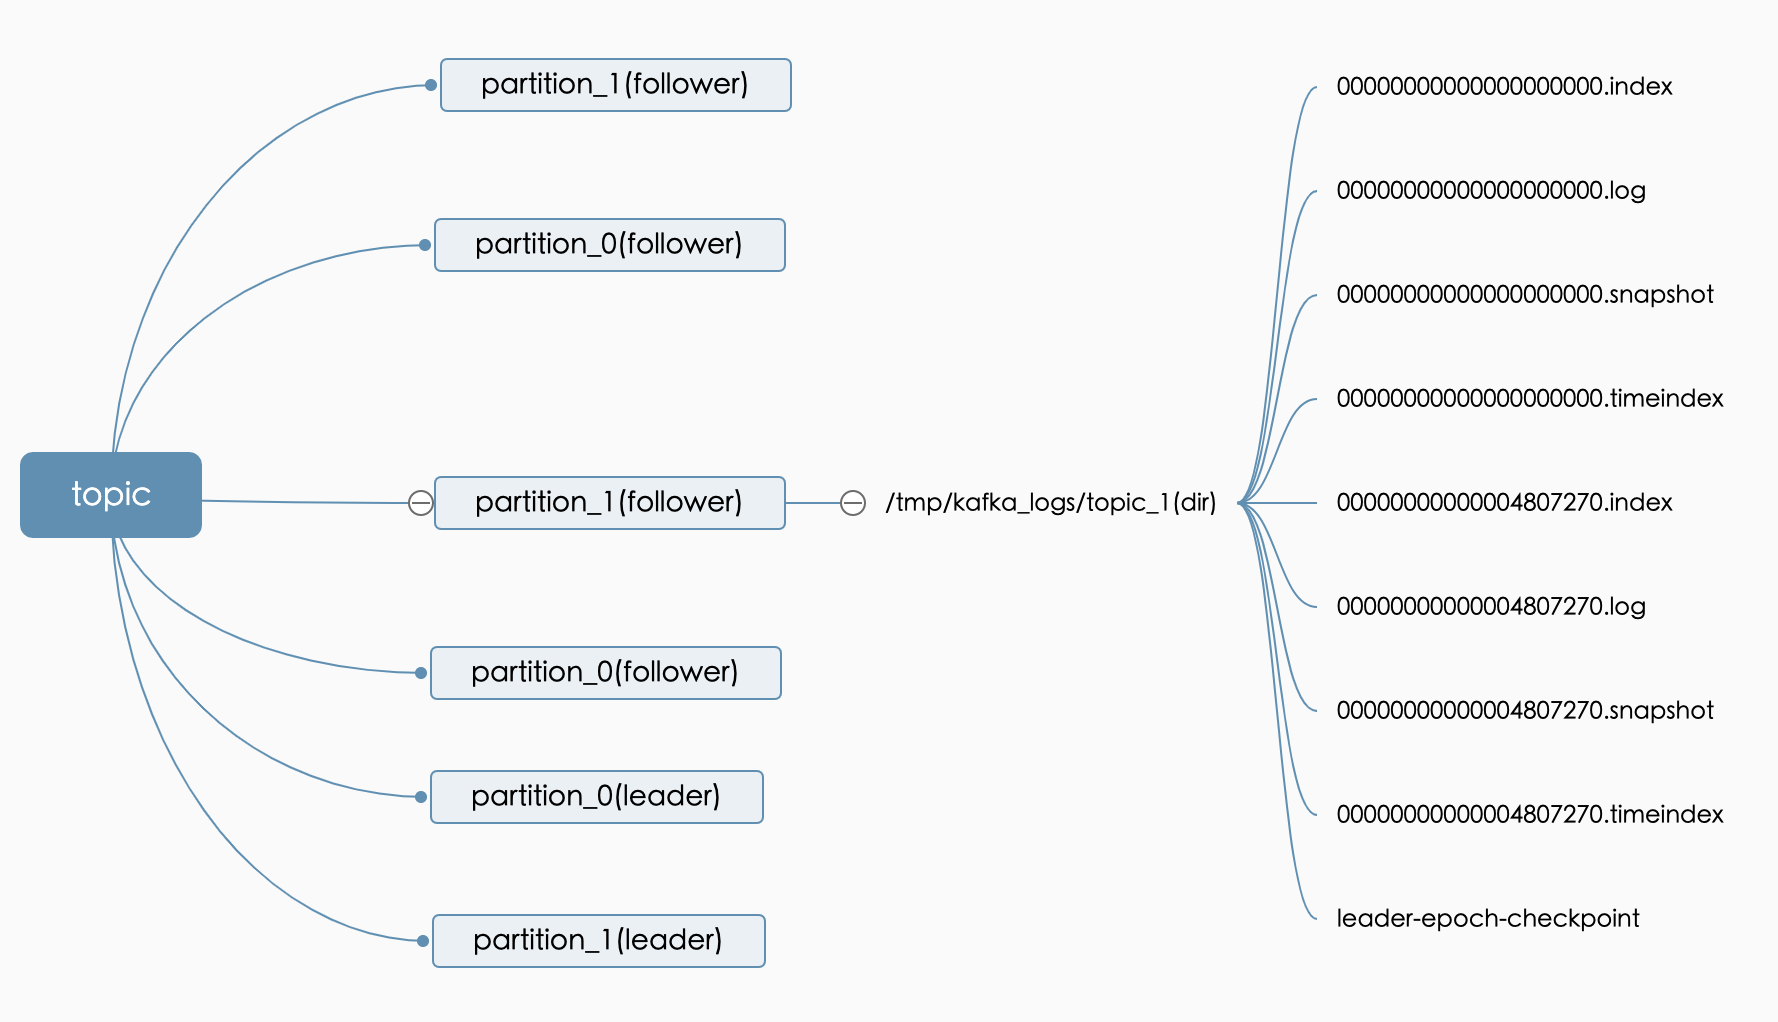
\includegraphics[width=0.9\linewidth]{image/0220}
    %\caption{}
    \label{fig:0220}
\end{figure}

\end{frame}

\begin{frame}[plain,t]{Broker} %也可以使用\frametitle{节的名字}效果一样
    \structure{Failover} \\
    \vspace{2ex}
    \begin{figure}
        \centering
        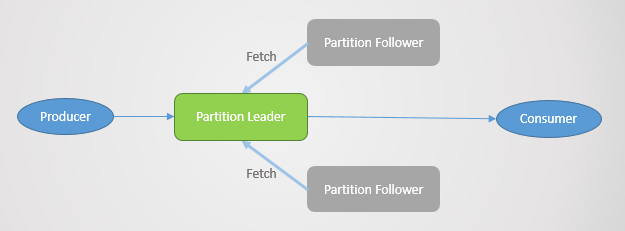
\includegraphics[width=0.8\linewidth]{image/0210}
        %\caption{}
        \label{fig:0210}
    \end{figure}
     \begin{figure}
        \centering
        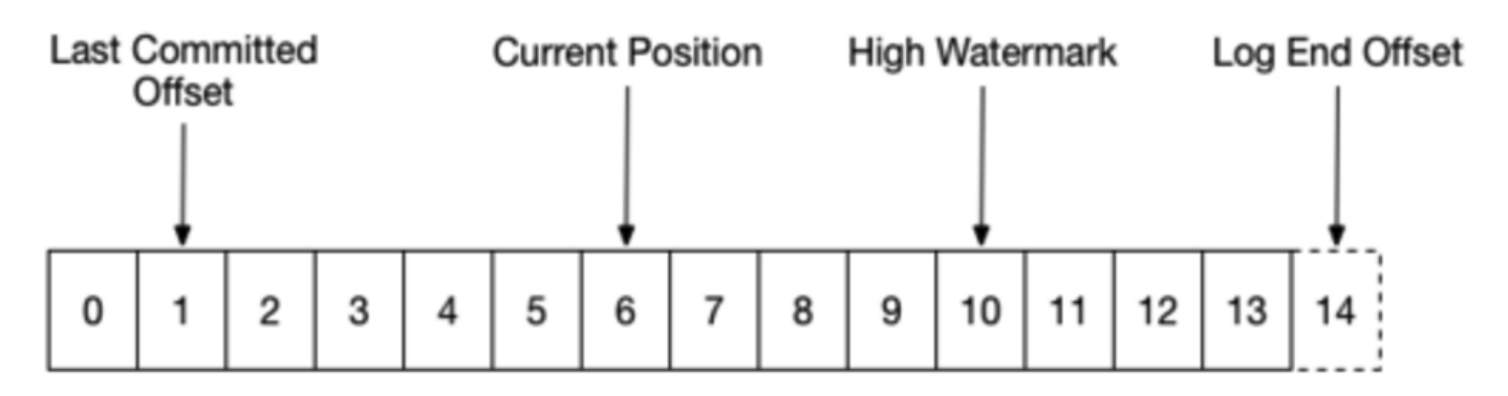
\includegraphics[width=0.85\linewidth]{image/0211}
        %\caption{}
        \label{fig:0211}
    \end{figure}
    
\end{frame}

\begin{frame}[plain,t]{Broker} %也可以使用\frametitle{节的名字}效果一样
    \structure{Why Kafka Is so Fast} \\
    \vspace{2ex}
    Kafka relies heavily on the filesystem for storing and caching messages. 
    
    \begin{figure}
        \centering
        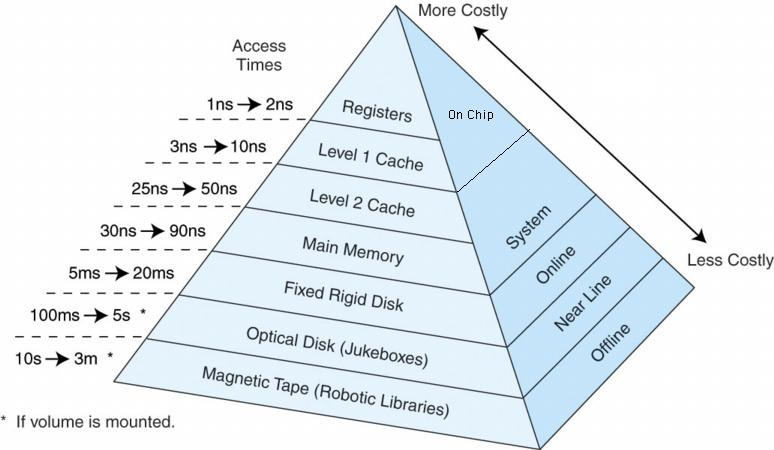
\includegraphics[width=0.8\linewidth]{image/0212}
        %\caption{}
        \label{fig:0212}
    \end{figure}
    
    
    
\end{frame}
\begin{frame}[plain,t]{Broker} %也可以使用\frametitle{节的名字}效果一样
    \structure{Why Kafka Is so Fast} \\
    \vspace{2ex}
      As a result the performance of linear writes on a JBOD configuration with six 7200rpm SATA RAID-5 array.
      \begin{itemize}
          \item linear writes 600MB/sec 
          \item random writes 100k/sec
      \end{itemize}
      
      
    
    \vspace{2ex}
    \begin{figure}
        \centering
        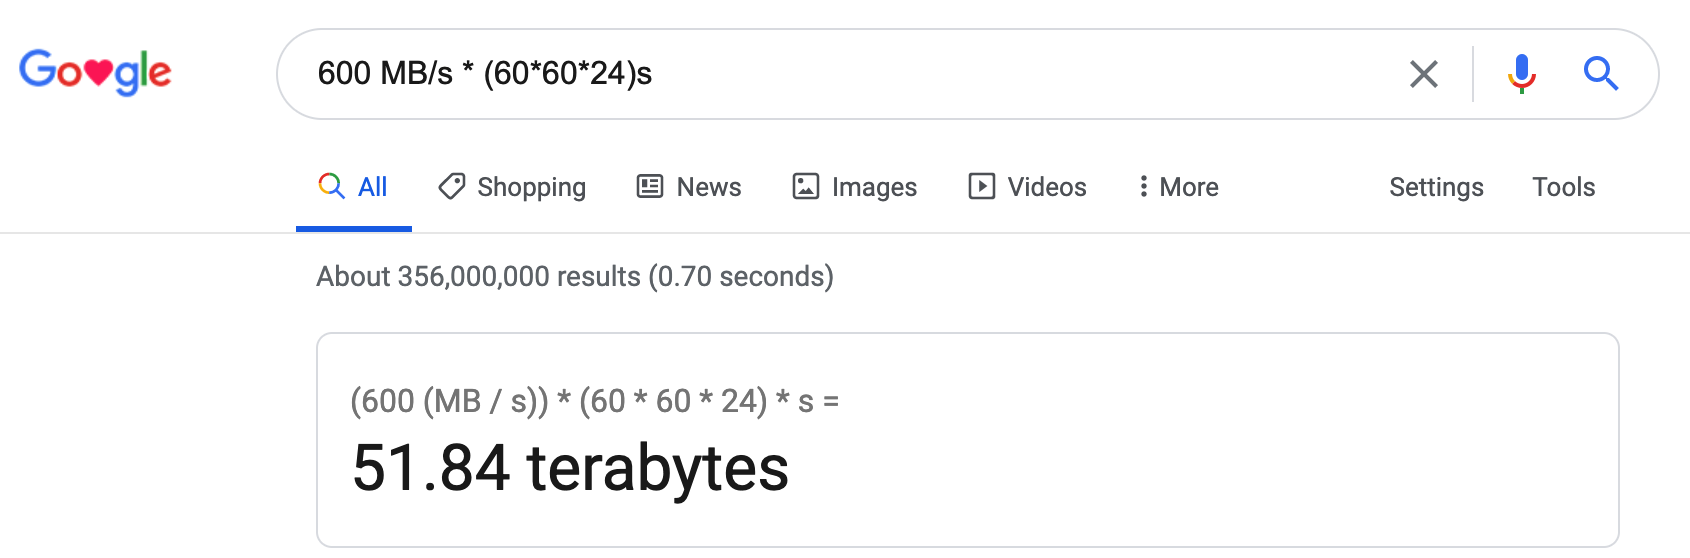
\includegraphics[width=0.9\linewidth]{image/0213}
        %\caption{}
        \label{fig:0213}
    \end{figure}
    
    
\end{frame}
\begin{frame}[plain,t]{Broker} %也可以使用\frametitle{节的名字}效果一样
    \structure{Why Kafka Is so Fast} \\
    \vspace{2ex}
     To illustrate the page cache, a Linux program named render, which opens file scene.dat and reads it 512 bytes at a time. 
    
    \begin{figure}
        \centering
        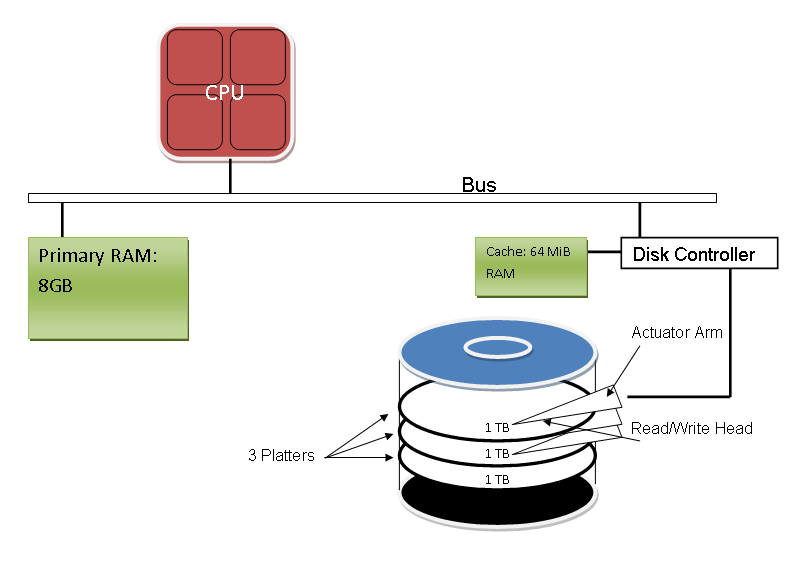
\includegraphics[width=0.7\linewidth]{image/0214}
        %\caption{}
        \label{fig:0214}
    \end{figure}
    
\end{frame}
\begin{frame}[plain,t]{Broker} %也可以使用\frametitle{节的名字}效果一样
    \structure{Why Kafka Is so Fast} \\
    \vspace{2ex}
    The first read goes like this:
    \begin{figure}
        \centering
        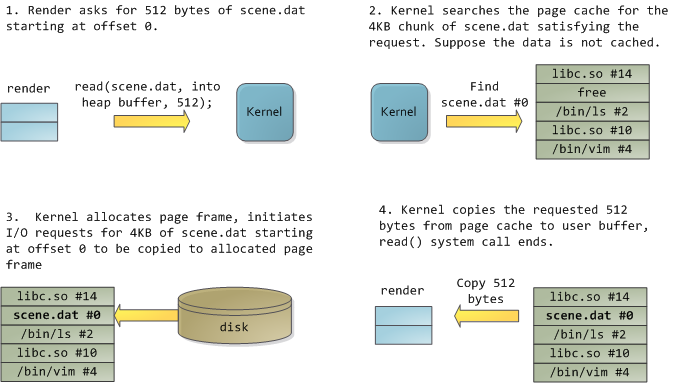
\includegraphics[width=0.9\linewidth]{image/0215}
        %\caption{}
        \label{fig:0215}
    \end{figure}
    
\end{frame}
\begin{frame}[plain,t]{Broker} %也可以使用\frametitle{节的名字}效果一样
    \structure{Why Kafka Is so Fast} \\
    \vspace{2ex}
     For  reuse, the kernel will use {\color{red}memory-mapped files} to map your program's virtual pages directly onto the page cache.
    
    \vspace{2ex}
    \begin{figure}
        \centering
        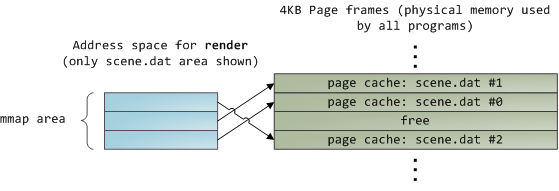
\includegraphics[width=0.9\linewidth]{image/0216}
        %\caption{}
        \label{fig:0216}
    \end{figure}
    
\end{frame}
\begin{frame}[plain,t]{Broker} %也可以使用\frametitle{节的名字}效果一样
    \structure{Why Kafka Is so Fast} \\
    \vspace{2ex}
    
Kafka are building on top of the JVM, and anyone who has spent any time with Java memory usage knows two things:
\vspace{2ex}
\begin{itemize}
    \item the memory overhead of objects is very high
    \item  java garbage collection becomes increasingly fiddly and slow as the in-heap data increases
\end{itemize}

\vspace{2ex}
Doing so will result in a cache of up to 28-30GB on a 32GB machine without GC penalties.


\end{frame}
\begin{frame}[plain,t]{Broker} %也可以使用\frametitle{节的名字}效果一样
    \structure{Why Kafka Is so Fast} \\
    \vspace{2ex}
Once poor disk access patterns have been eliminated, there are two common causes of inefficiency in this type of system:
\vspace{2ex}
\begin{enumerate}
    \item too many small I/O operations
    \begin{itemize}
        \item batch
        \item compression
    \end{itemize}
    \item excessive byte copying
    \begin{itemize}
        \item a standardized binary message format
        \item zero copy
    \end{itemize}
\end{enumerate}


\end{frame}
\begin{frame}[plain,t]{Broker} %也可以使用\frametitle{节的名字}效果一样
    \structure{Why Kafka Is so Fast} \\
    %\vspace{2ex}
 \begin{figure}
    \centering
    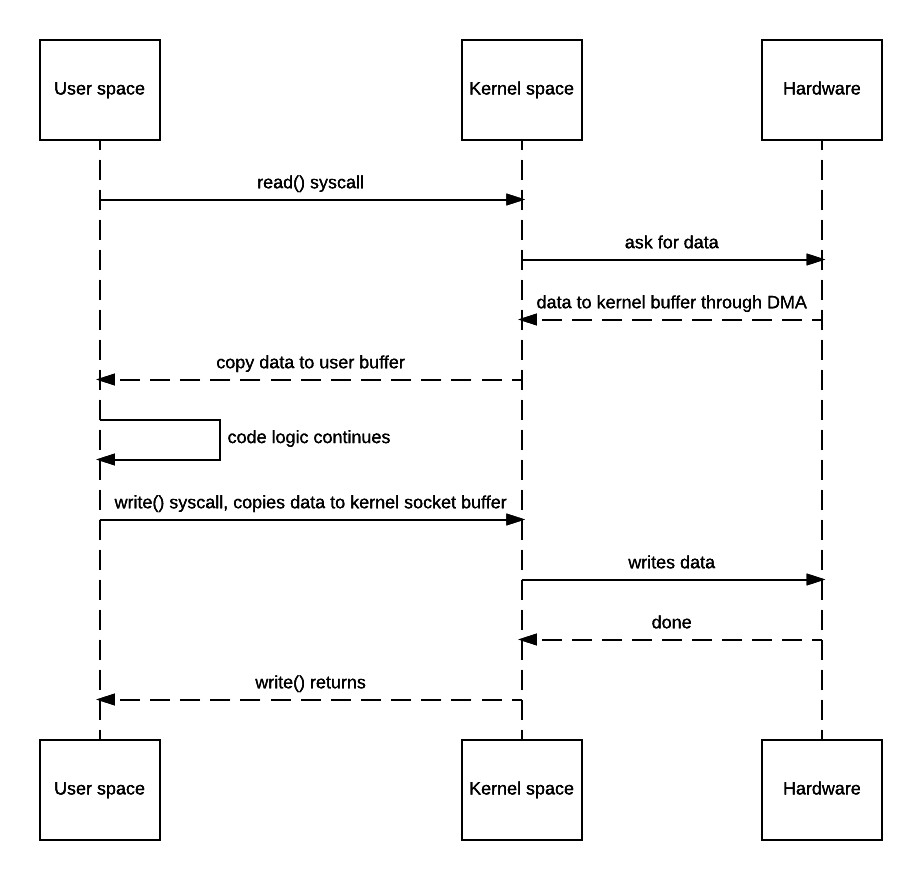
\includegraphics[width=0.7\linewidth]{image/0201}
    %\caption{}
    \label{fig:0201}
\end{figure}
\end{frame}
\begin{frame}[plain,t]{Broker} %也可以使用\frametitle{节的名字}效果一样
    \structure{Why Kafka Is so Fast} \\
    %\vspace{2ex}
    \begin{figure}
        \centering
        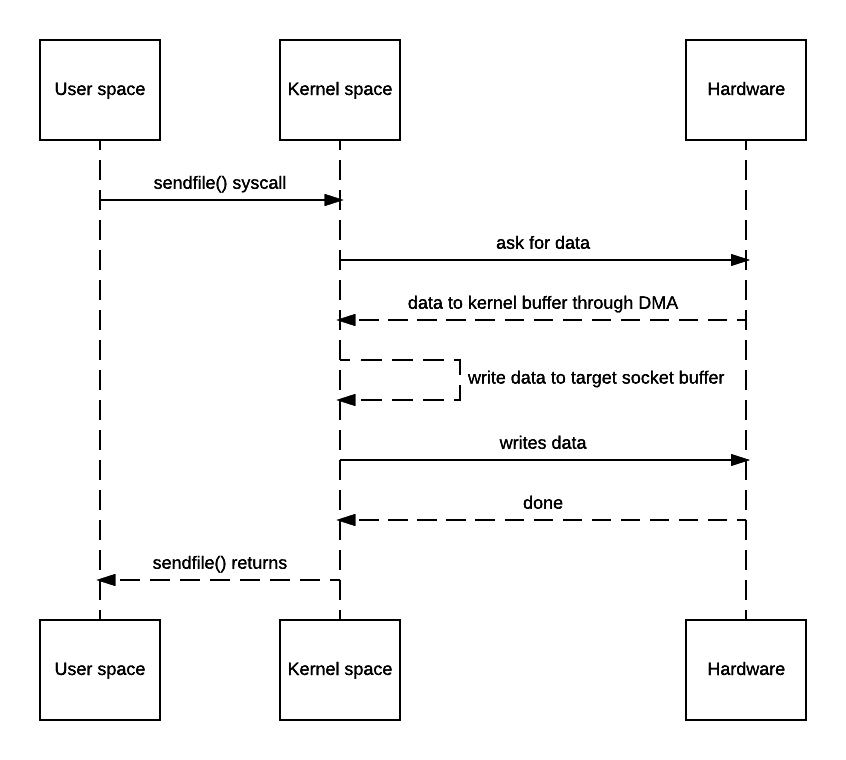
\includegraphics[width=0.7\linewidth]{image/0202}
        %\caption{}
        \label{fig:0202}
    \end{figure}
    
\end{frame}
\begin{frame}[plain,t]{Broker} %也可以使用\frametitle{节的名字}效果一样
    \structure{Why Kafka Is so Fast} \\
    %\vspace{2ex}
    
    \begin{figure}
        \centering
        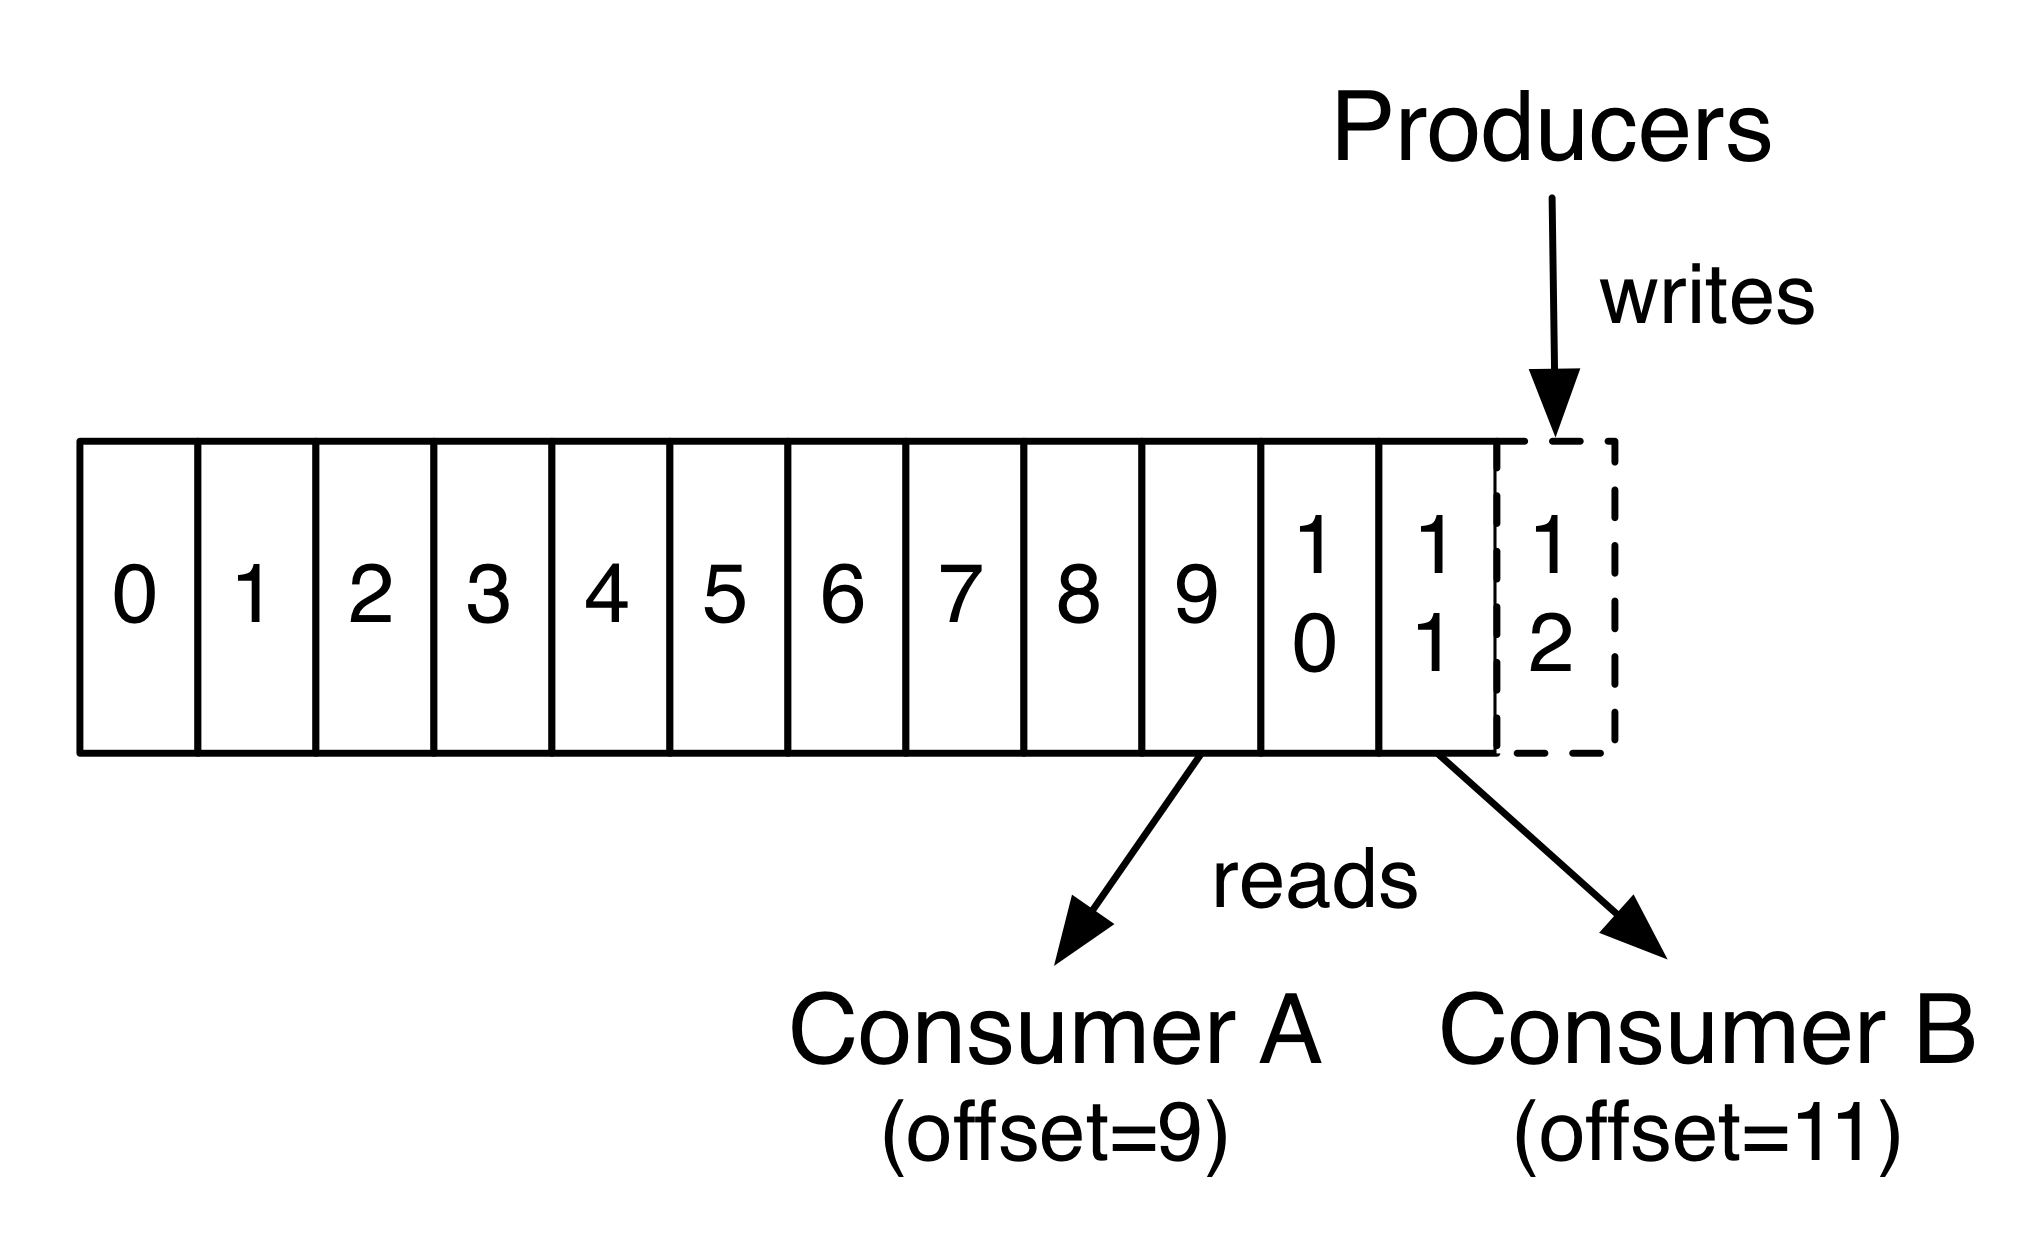
\includegraphics[width=0.9\linewidth]{image/0104}
        %\caption{}
        \label{fig:0104}
    \end{figure}
    
\end{frame}
\section{Consumer}

\begin{frame}[plain,t]{Consumer} %也可以使用\frametitle{节的名字}效果一样
    \structure{Consumer Groups} \\
    \vspace{2ex}
     \begin{figure}
        \centering
        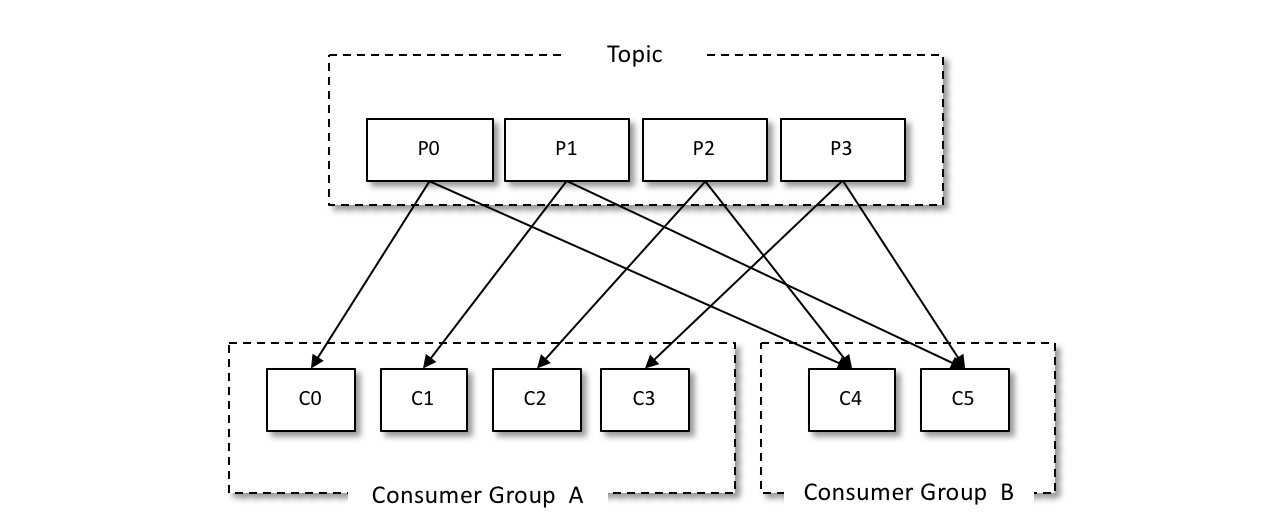
\includegraphics[width=0.9\linewidth]{image/0205}
        %\caption{}
        \label{fig:0205}
    \end{figure}
    
    
\end{frame}
\begin{frame}[plain,t]{Consumer} %也可以使用\frametitle{节的名字}效果一样
    \structure{Consumer Groups} \\
    \vspace{2ex}
    \begin{figure}
        \centering
        \subcaptionbox{group rebalance }{
            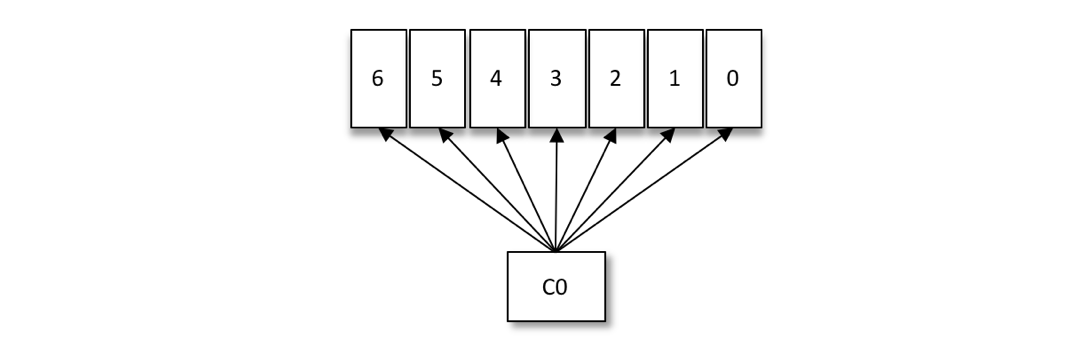
\includegraphics[width=0.48\linewidth]{image/0206}\quad
            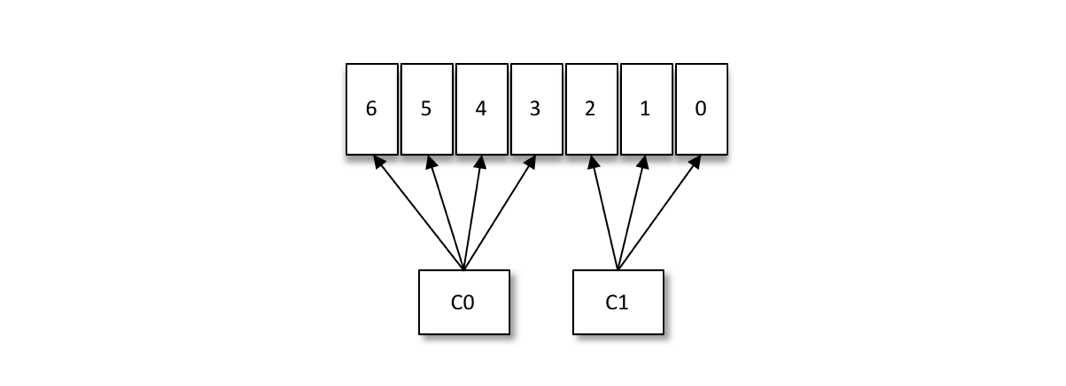
\includegraphics[width=0.48\linewidth]{image/0207}
        }
    \subcaptionbox{group rebalance}{
        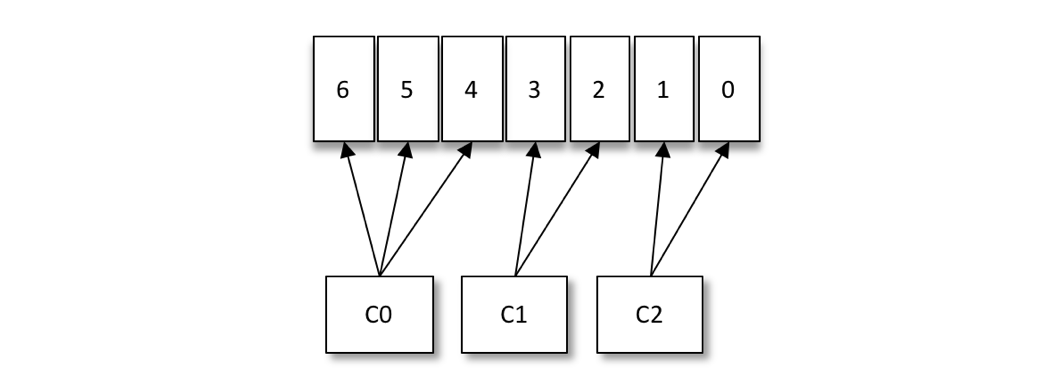
\includegraphics[width=0.48\linewidth]{image/0208}\quad
        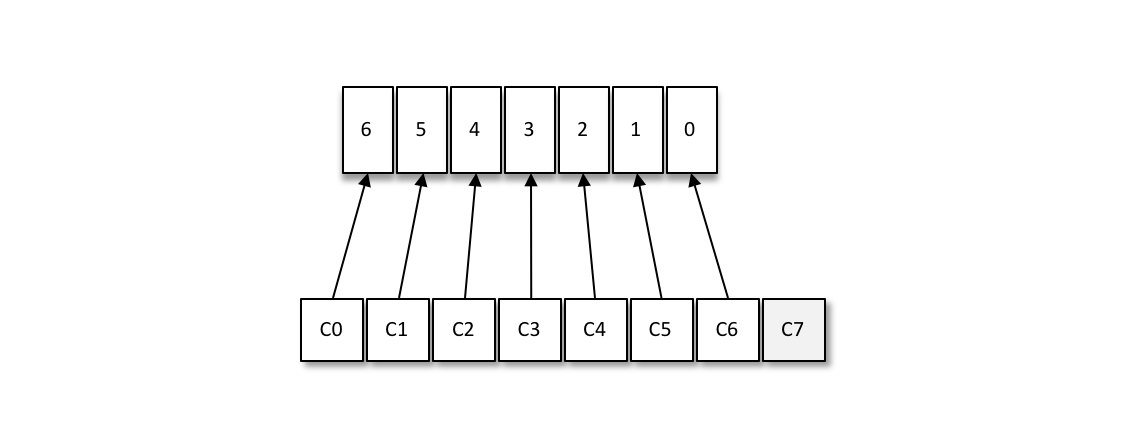
\includegraphics[width=0.48\linewidth]{image/0209}
    }
    
    
        
        %\caption{}
        \label{fig:0101}
    \end{figure}
    
\end{frame}
\begin{frame}[plain,t]{Consumer} %也可以使用\frametitle{节的名字}效果一样
    \structure{Offsets and Consumer Position} \\
    \vspace{2ex}
    
    
    \begin{figure}
        \centering
        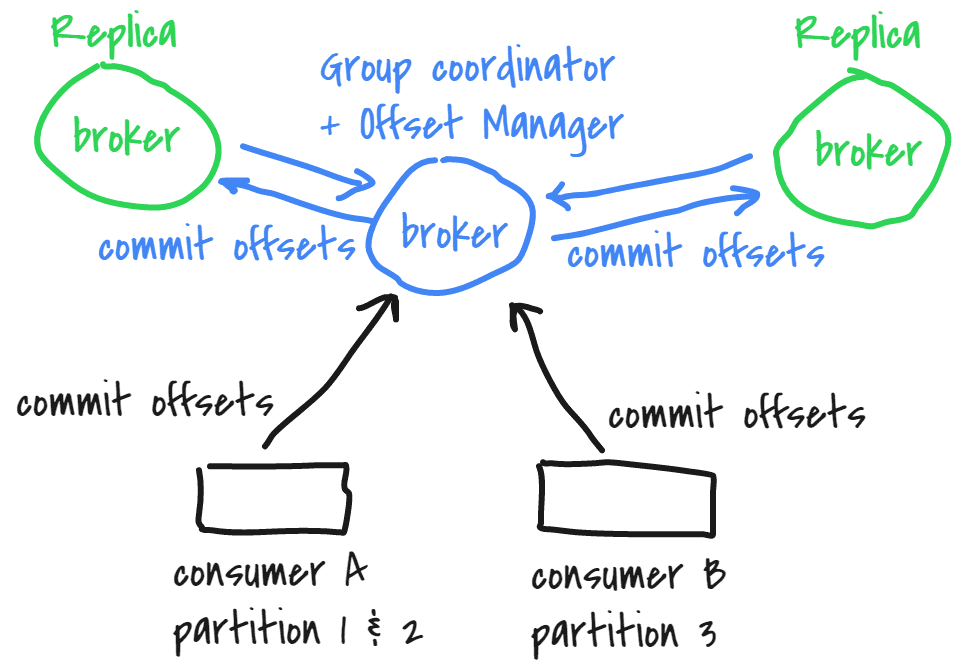
\includegraphics[width=0.7\linewidth]{image/0306}
        %\caption{}
        \label{fig:0306}
    \end{figure}
    
\end{frame}
\begin{frame}[plain,t]{Consumer} %也可以使用\frametitle{节的名字}效果一样
    \structure{Offsets and Consumer Position} \\
    \vspace{2ex}

    \begin{figure}
        \centering
        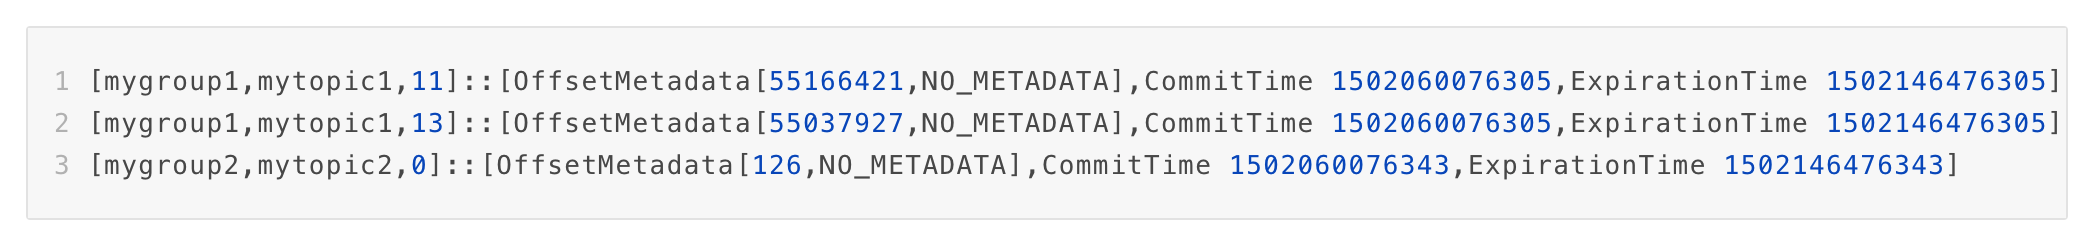
\includegraphics[width=1\linewidth]{image/0219}
        %\caption{}
        \label{fig:0219}
    \end{figure}
    \begin{figure}
        \centering
        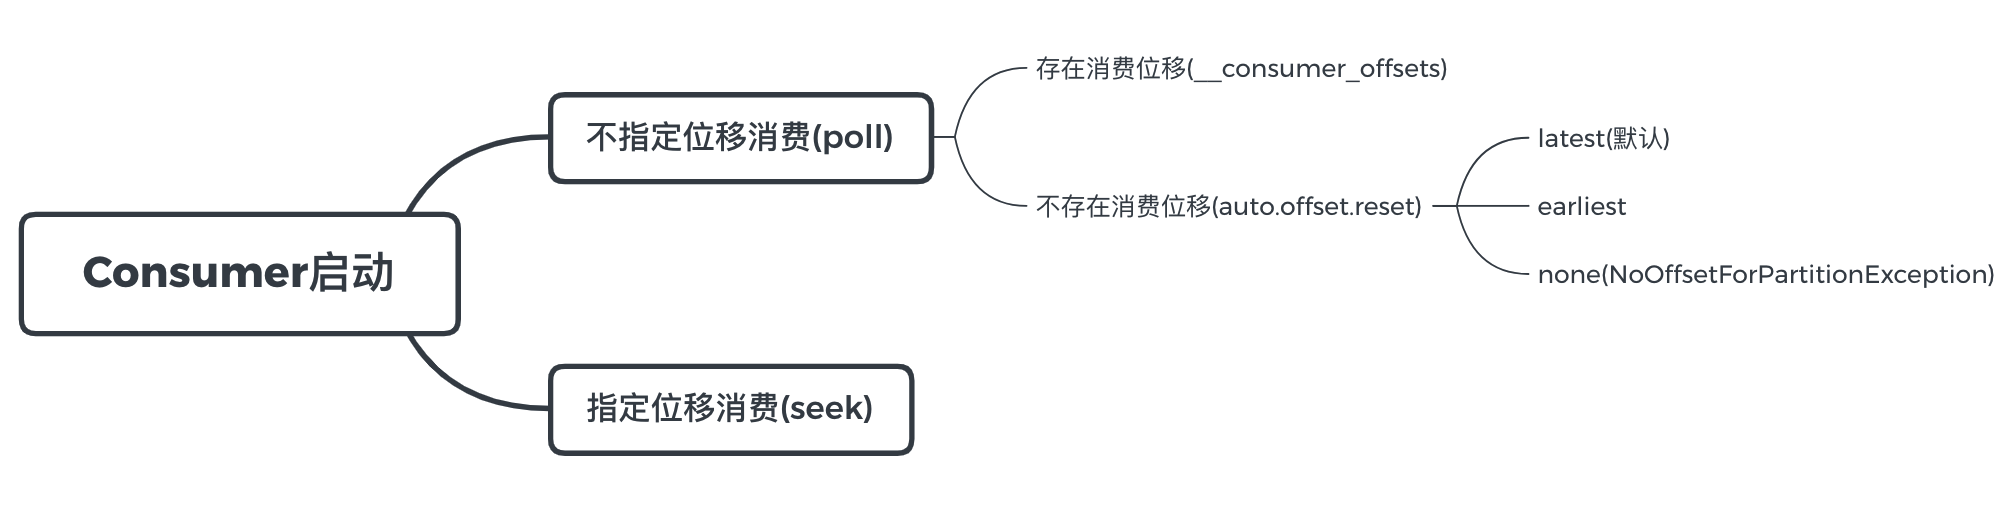
\includegraphics[width=0.9\linewidth]{image/0217}
        %\caption{}
        \label{fig:0217}
    \end{figure}
\end{frame}

\begin{frame}[plain,t]{Consumer} %也可以使用\frametitle{节的名字}效果一样
    \structure{Storing Offsets Outside Kafka} \\
    \vspace{2ex}
    The application can store both the offset and the results of the consumption in the same system.
    
    \vspace{2ex}
    It will make the consumption fully atomic and give "exactly once" semantics.
    
    \vspace{2ex}
    Each record comes with its own offset, so to manage your own offset:
    \begin{itemize}
        \item configure enable.auto.commit=false
        \item use each offset to save your position
        \item on restart restore the position of the consumer using seek()
    \end{itemize}
    
    
\end{frame}





%%=================================================================================================
\begin{frame}[plain]
    \huge
    \vfill
    \centerline{ \structure{Questions and Answers?} }
    \vfill
    
\end{frame}
\begin{frame}[plain]
    \huge
    \vfill
    \centerline{ \structure{Questions and Answers?} }
    \vfill
    \Huge
    \centerline{\alert{Thank You!} }
    \vfill
\end{frame}

%**********************************************************************************************
%                  上面就是正文,自己的内容
%        下面是标准的参考文献配置
%**********************************************************************************************
\begin{frame}[plain, t, allowframebreaks]{References}
    %  allowframebreaks,这个关键字可以使得参考文献自动断页,免得手动
    %  plain格式使得一帧的最上面是白色的,没有plain,会有色彩,可以试试
    %  t 使得正文不再是默认居中,而是在top,应该加上t,比较好看。
    \bibliographystyle{alpha}         %文献的格式apalike是[1],alpha是[Lam94]
    %\beamertemplatetextbibitems        %调整文献样式
    %\scriptsize                        %文献多时调整字体大小
    %\bibliography{math}                 %自己的文献
\end{frame}  



\end{document} 
%**********************************************************************************************
%        上面是标准的参考文献配置
%   参考文献的主题选择apalike,见《LaTeX入门》作者:刘海洋P423页(6-1-13)说明
%   apalike文献格式,按照美国心理协会(APA)的格式,提供基本的作者年代引用方式
%   避免完全不直观的数学编号可能造成的问题。这是因为beamer的文献格式比较特殊造成的
%  实例如下:
%\beamertemplatetextbibitems %该指令可使参考文献采用文字而不是图标的标注
%\begin{frame}[plain, t, allowframebreaks]{References}
%	\scriptsize
%	\bibliographystyle{apalike}
%	\bibliography{ZhangXiao-Smoothed_Analysis_of_Tensor_Decompositions} %文献命名规范,不要怕长
%\end{frame}

%**********************************************************************************************
%   学习LaTeX好的资料,有《LaTeX入门》《A Guide to LaTeX 4th Edition》 新浪微盘可下载  
%   《一份不太简短的LATEX介绍 》,网址 CTAN:/tex-archive/info/lshort 可下载  ,有中英文,每年更新
%   tex.stackexchange.com,一个美国的专业TeX问答网站,这个网站更灵活,受益匪浅
%   www.ctan.org            usepackage资料参考
%   www.texample.net       不常用,但是聚集了的专业绘图的LaTeX代码,比如画一个probability tree,
%   遇到问题,先百度Google,90%问题可解决,不行再上知乎提问,刘海洋老师,LaTeX专家,
%   可在 tex.stackexchange.com  同时提问,最基础的是读读上面的两本书,学会自己看文档
%   论文《Type setting mathematics for science and technology according to ISO 31/XI》
%   介绍排版中数学字体的选择
%***********************************************************************************************
